%! Author = gramic
%! Date = 08.05.24

% Preamble
\begin{flushleft}
    \section{Monitoring}
    Das Monitoring im \Gls{PRTG} besteht aus zwei Teilen.\\
    Zum einen werden die Standard-Werte wie Ping, CPU Load, Load Average, Disk Free, Traffic und die Uptime:
    \begin{figure}[H]
        \centering
        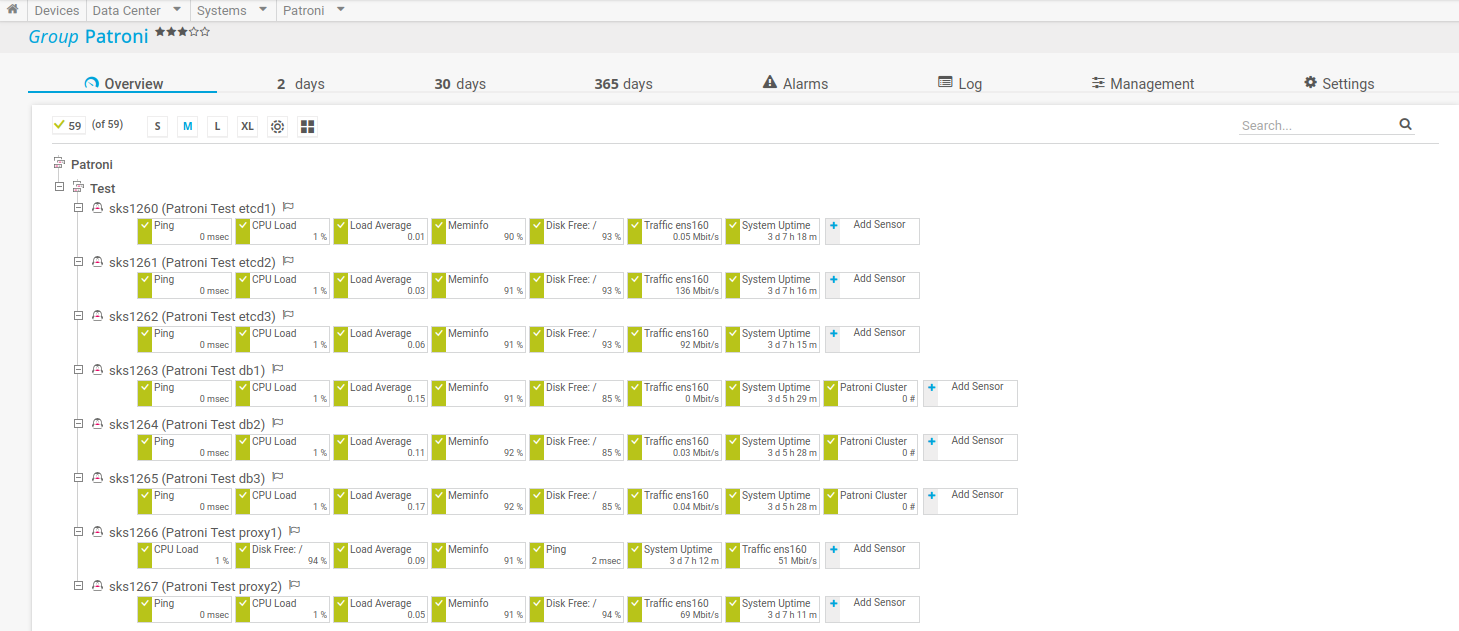
\includegraphics[width=1\linewidth]{source/implementation/construction_implementation/monitoring/prtg_patroni}
        \caption{\Gls{PRTG} - Patroni Monitoring}
        \label{fig:prtg_patroni}
    \end{figure}
\end{flushleft}
\begin{flushleft}
    Zusätzlich wurde ein Python Custom Sensor erstellt.\\
    Dieser nutzt die Patroni REST-API um folgende Werte abzufragen:
    \begin{description}
        \item \textbf{Cluster Status}\hfill \\Prüft, ob der Cluster noch im Status running ist.\\Dabei wird geprüft ob der Cluster \guillemotleft running\guillemotright ist.\\Ist der Cluster pausiert, wird eine Warnung ausgegeben.\\Andernfalls wird ein Fehler geworfen.
        \item \textbf{Cluster Unlock}\hfill \\Ein Patroni Node kann nur Primary werden, wenn im DCS (in diesem Fall \gls{etcd}) der Leader-Lock gesetzt werden kann.\\In diesem Fall wird ein Fehler geworfen.
        \item \textbf{Failsafe Mode Activity}\hfill \\Zusätzlich kann der \guillemotleft\texttt{failsafe\_mode}\guillemotright aktiviert werden.\\Dann kann \Gls{PostgreSQL} trotzdem als Primary Node laufen\cite{KFMY83EB}.
        \item \textbf{Replication Lag}\hfill \\Prüft, ob das Replication Lag unterhalb dem Übergebenen Wert liegt.\\Es gibt eine Abfrage für die Warngrenze und eine Fehlergrenze.
        \item \textbf{Replication State}\hfill \\Liest die States der Replikas aus.\\Dabei wird eine Warnung ausgegeben, wenn nicht alle Nodes im \guillemotleft\texttt{sync}\guillemotright Mode sind.\\Ein Fehler wird ausgegeben wenn keiner der Patrroni Nodes in diesem State ist.
    \end{description}
\end{flushleft}
\begin{flushleft}
    Die Konfiguration wird im \Gls{PRTG} gemacht.\\
    Dabei müssen im Feld \guillemotleft\texttt{Additional Parameters}\guillemotright folgende Parameter übergeben werden:
    \begin{description}
        \item \textbf{replication\_mode}\hfill \\Der Replikationsmodus.\\Für diesen Cluster ist es \guillemotleft\texttt{sync}\guillemotright für synchrone Replikation.
        \item \textbf{lag\_warning}\hfill \\Wenn das Replication Lag 2GB übersteigt, wird eine Warnung ausgeworfen.
        \item \textbf{lag\_error}\hfill \\Wenn das Replication Lag 4GB übersteigt, wird ein Fehler.
    \end{description}
    Die Werte werden Kommasepariert übergeben:\\
    \texttt{replication\_mode=sync,lag\_warning=2GB,lag\_error=4GB}
    \begin{figure}[H]
        \centering
        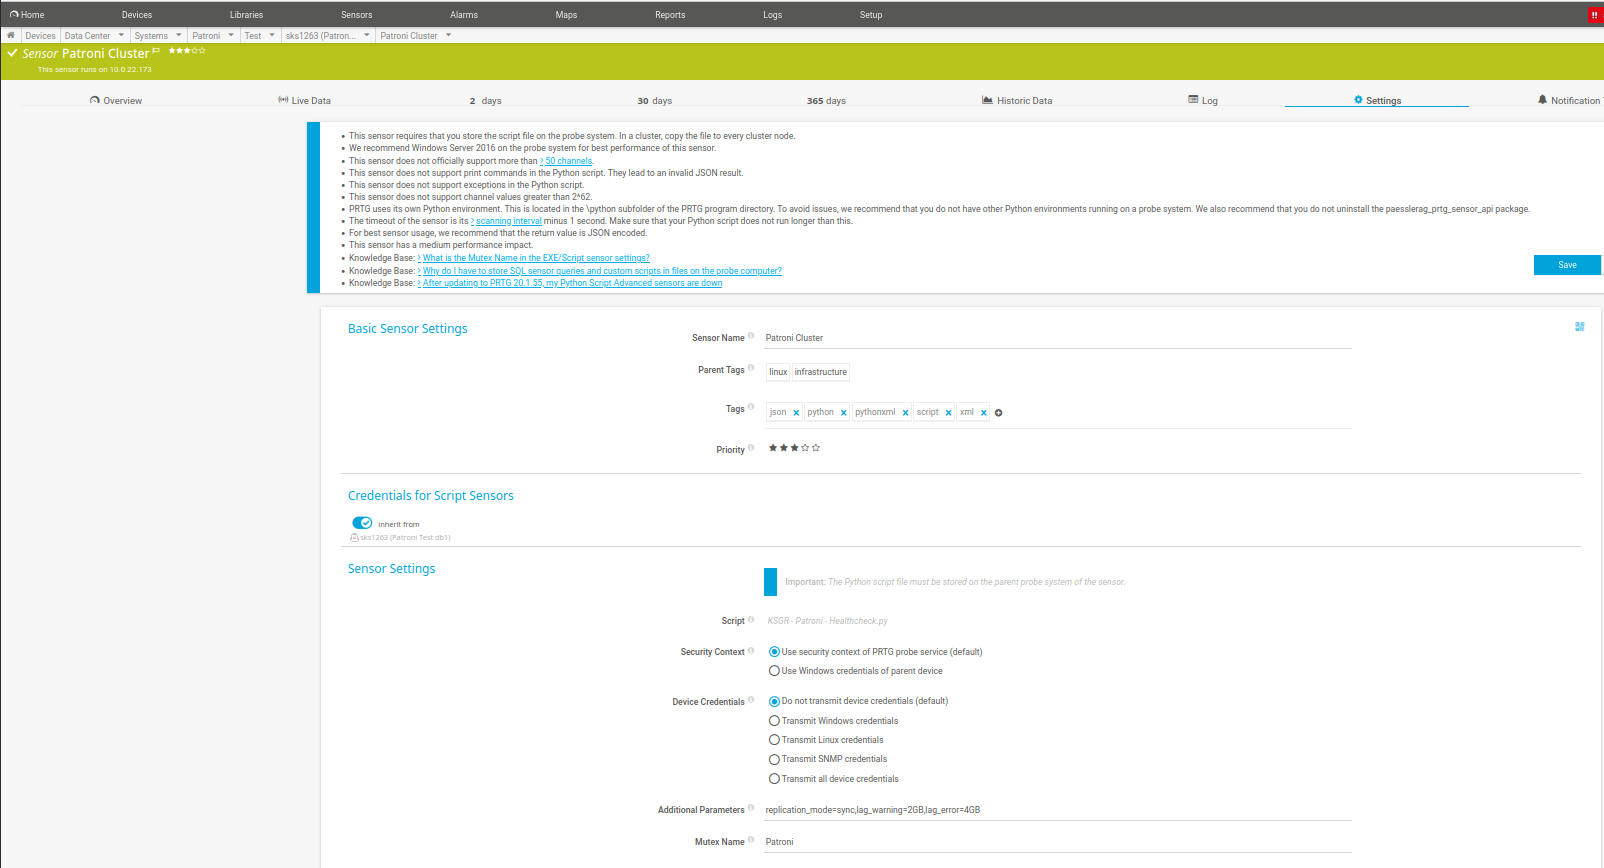
\includegraphics[width=1\linewidth]{source/implementation/construction_implementation/monitoring/patroni_cluster_sensor_setting}
        \caption{\Gls{PRTG} - Patroni Cluster Sensor Setting}
        \label{fig:patroni_cluster_sensor_setting}
    \end{figure}
\end{flushleft}
\begin{flushleft}
    Der Sensor sieht im \Gls{PRTG} dann so aus:
    \begin{figure}[H]
        \centering
        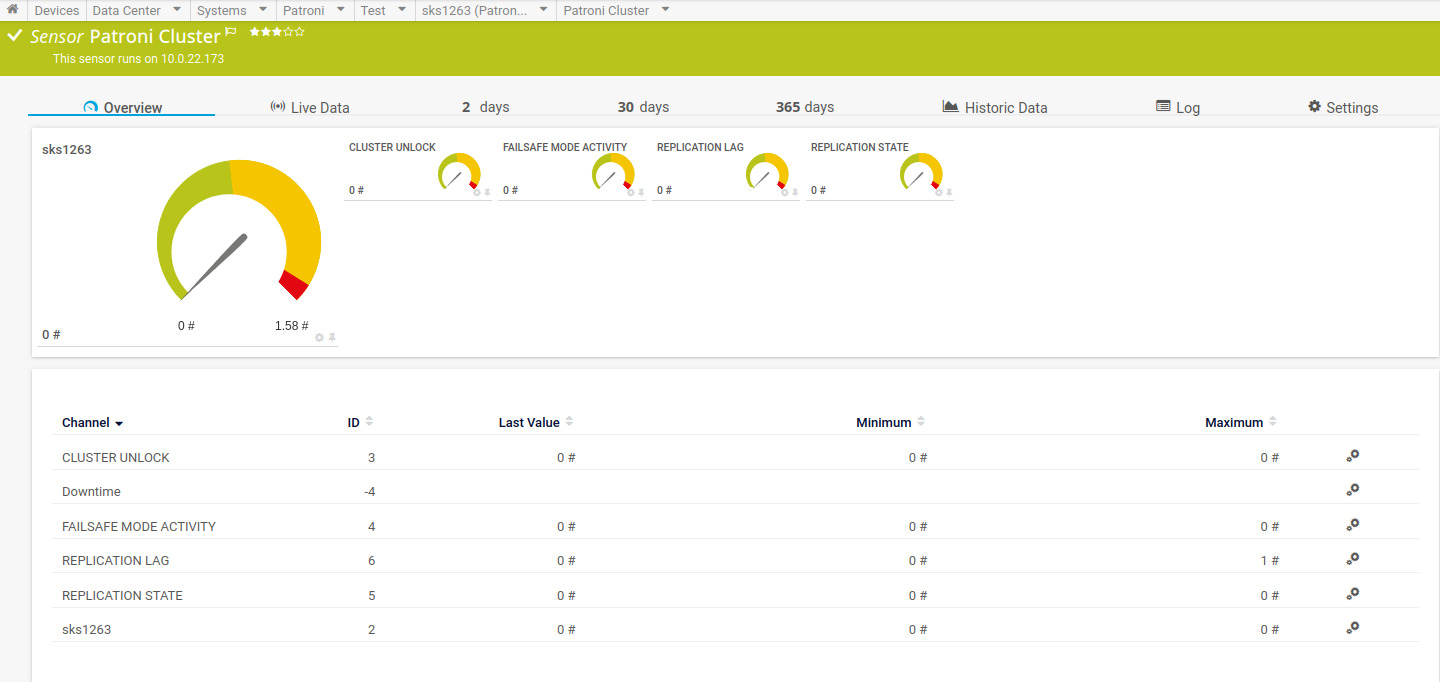
\includegraphics[width=1\linewidth]{source/implementation/construction_implementation/monitoring/patroni_cluster_sensor}
        \caption{\Gls{PRTG} - Patroni Cluster Sensor}
        \label{fig:patroni_cluster_sensor}
    \end{figure}
\end{flushleft}